\begin{exo}[Des cubes ...]
	Cette figure montre la décomposition en plusieurs solides d'un cube d'arête $a + b$ où $a$ et $b$ sont des nombres réels positifs.

	\begin{center}
		\definecolor{cubevert}{RGB}{160,200,30}
		\definecolor{cubeorange}{RGB}{250,185,40}
		\definecolor{cubebleu}{RGB}{50,170,200}
		\definecolor{cuberouge}{RGB}{225,85,35}
		\newcommand{\boite}[7]{%
			{\pgfmathsetmacro{\xb}{#1+#4}%
					\pgfmathsetmacro{\yb}{#2+#5}%
					\pgfmathsetmacro{\zb}{#3+#6}%
					\filldraw[fill=#7!70!white, draw=white, line join=round, line width=0.4pt]
					(#1,#2,\zb) -- (\xb,#2,\zb) -- (\xb,\yb,\zb) -- (#1,\yb,\zb) -- cycle;
					\filldraw[fill=#7, draw=white, line join=round, line width=0.4pt]
					(\xb,#2,#3) -- (\xb,\yb,#3) -- (\xb,\yb,\zb) -- (\xb,#2,\zb) -- cycle;
					\filldraw[fill=#7!75!black, draw=white, line join=round, line width=0.4pt]
					(#1,\yb,#3) -- (\xb,\yb,#3) -- (\xb,\yb,\zb) -- (#1,\yb,\zb) -- cycle;}%
		}

		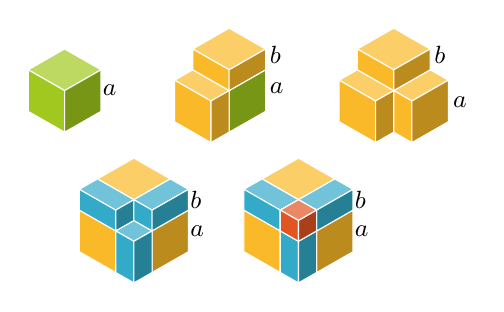
\begin{tikzpicture}[scale=1.1, x={(-0.21cm,-0.12cm)}, y={(0.21cm,-0.12cm)}, z={(0cm,0.24cm)}, font=\small]
			\begin{scope}
				\boite{0}{0}{0}{2}{2}{2}{cubevert}
				\node[right=-1mm] at (0,2,1) {$a$};
			\end{scope}
			\begin{scope}[xshift=1.9cm]
				\boite{0}{0}{0}{2}{2}{2}{cubevert}
				\boite{2}{0}{0}{1}{2}{2}{cubeorange}
				\boite{0}{0}{2}{2}{2}{1}{cubeorange}
				\node[right=-3mm] at (0,3,3.2) {$b$};
				\node[right=-3mm] at (0,3,1.6) {$a$};
			\end{scope}
			\begin{scope}[xshift=3.8cm]
				\boite{2}{0}{0}{1}{2}{2}{cubeorange}
				\boite{0}{2}{0}{2}{1}{2}{cubeorange}
				\boite{0}{0}{2}{2}{2}{1}{cubeorange}
				\node[right=-3mm] at (0,3,3.2) {$b$};
				\node[right=1mm] at (0,2.3,0.6) {$a$};
			\end{scope}
			\begin{scope}[xshift=0.8cm, yshift=-1.5cm]
				\boite{2}{0}{0}{1}{2}{2}{cubeorange}
				\boite{0}{2}{0}{2}{1}{2}{cubeorange}
				\boite{0}{0}{2}{2}{2}{1}{cubeorange}
				\boite{2}{2}{0}{1}{1}{2}{cubebleu}
				\boite{2}{0}{2}{1}{2}{1}{cubebleu}
				\boite{0}{2}{2}{2}{1}{1}{cubebleu}
				\node[right=-1mm] at (0,3,2.5) {$b$};
				\node[right=-1mm] at (0,3,1)   {$a$};
			\end{scope}
			\begin{scope}[xshift=2.7cm,yshift=-1.5cm]
				\boite{2}{0}{0}{1}{2}{2}{cubeorange}
				\boite{0}{2}{0}{2}{1}{2}{cubeorange}
				\boite{0}{0}{2}{2}{2}{1}{cubeorange}
				\boite{2}{2}{0}{1}{1}{2}{cubebleu}
				\boite{2}{0}{2}{1}{2}{1}{cubebleu}
				\boite{0}{2}{2}{2}{1}{1}{cubebleu}
				\boite{2}{2}{2}{1}{1}{1}{cuberouge}
				\node[right=-1mm] at (0,3,2.5) {$b$};
				\node[right=-1mm] at (0,3,1)   {$a$};
			\end{scope}
		\end{tikzpicture}
	\end{center}

	\begin{enumerate}
		\item Pour chaque couleur de solide (vert, jaune, bleu et rouge) :
		      \begin{enumerate}
			      \item Déterminer le nombre de solides.
			      \item Déterminer le volume d'un solide en fonction de $a$ et $b$.
		      \end{enumerate}
		\item Montrer que $(a + b)^3 = a^3 + 3a^2b + 3ab^2 + b^3$.
		\item Cette égalité est-elle démontrée pour tous $a$ et $b$ ?
	\end{enumerate}
\end{exo}
